% **************************** %
%          Slides GK           %
% **************************** %

\documentclass[10pt,fleqn]{beamer}
 
% **************************** %
%            Package           %
% **************************** %
% \usepackage{GarmirKhatch}
\usepackage[utf8]{inputenc}
\usepackage[T1]{fontenc}
\usepackage[french,english]{babel}
\usepackage[french]{layout}
\usepackage{lmodern}
\usepackage{ragged2e}
\usepackage{fancyhdr}
\usepackage{verbatim}
\usepackage{graphicx}
\usepackage{wrapfig}
\usepackage{url}
\usepackage{hyperref}
\usepackage{amsmath}
\usepackage{multirow}
\usepackage{multicol}
\usepackage{array}
\usepackage{colortbl}
\usepackage{comment}
\usepackage{tikz}
\usetikzlibrary{positioning, shadows}

\newcommand{\mo}{\textsc{Garmir~Khatch}}

% **************************** %
%          Préambule           %
% **************************** %
% Option pdf
\hypersetup{
      %pdfpagemode = FullScreen,
      pdfauthor   = {AMU FSI 2014},
      pdftitle    = {Présentation du projet TMS pour \mo},
      pdfsubject  = {Système de gestion des transports},
      pdfkeywords = {AMO, GK, TMS, CdC, DAT, PTI}
}
% Thème du pdf 
\usetheme{Warsaw}
% Logo de l'université d'Aix-Marseille
%\logo{\includegraphics[height=6mm]{logo}}
% Affiche les notes
%\setbeameroption{show notes}
% Blocks arrondies et ombrés
\setbeamertemplate{blocks}[rounded][shadow=true] 
% Balle pour la liste d'items
\setbeamertemplate{itemize item}[ball]
% Triangle pour la liste de sous items
\setbeamertemplate{itemize subitem}[triangle]
% Affiche l'ensemble du frame en gris clair
\beamertemplatetransparentcovered
% Faire apparaître un sommaire avant chaque section
\AtBeginSection[]{
	\begin{frame}
		\frametitle{Sommaire}
		\tableofcontents[currentsection, hideallsubsections]
	\end{frame}
}

% **************************** %
%        Page de garde         %
% **************************** %
\title[]{{\Large \textsc{\mo \\ Système de gestion des transports}}}
\author[\textsc{\mo - Système de gestion des transports}]{M2 FSIL - FSI}
\institute{Encadrant : M. Roland \textsc{Agopian}\\
Faculté des Sciences d'Aix-Marseille Université\\
Campus de Luminy}
\date{\scriptsize{ 27 mars 2014}}

% **************************** %
%       Corps du document      %
% **************************** %
\begin{document}
 
% **************************** %
%            Entête            %
% **************************** %
\begin{frame}
\begin{figure}
\centering

\includegraphics[scale=0.52]{Images/EnTeteSciences}
\end{figure}
\titlepage
\end{frame}

\begin{frame}
\frametitle{Sommaire}
\tableofcontents[hideallsubsections]
\end{frame}

\section[Mission d'AMO~: recueil des besoins (CdCF)]{Mission d'AMO~: recueil des besoins (CdCF)}

\subsection[Compréhension du contexte]{Compréhension du contexte}
\begin{frame}
\end{frame}

\subsection[Compréhension des besoins]{Compréhension des besoins}
\begin{frame}
\end{frame}

\section[Mission de maîtrise d'œuvre~: réalisation du projet]{Mission de maîtrise d'œuvre~: réalisation du projet}

\subsection[Organisation (PAQ)]{Organisation (PAQ)}
\begin{frame}
\end{frame}

\subsection[Réponse technique aux besoins fonctionnels (DAT)]{Réponse technique aux besoins fonctionnels (DAT)}
\begin{frame}
\frametitle{}
\begin{block}{\textbf{Qu'est-ce que \mo~?}}
\begin{itemize}
\item Organisation humanitaires (187 Sociétés Nationales)
\item Vient en aide aux personnes plus vulnérables
\item Fort réseau de volontaires
\item Rend les communautés plus résistantes
\end{itemize}
\end{block}
\end{frame}

\subsection[Authentification et contrôle d'accès (LDAP)]{Authentification et contrôle d'accès (LDAP)}
\begin{frame}
  \frametitle{Authentification et contrôle d'accès}
  \begin{block}{\textbf{ Sommaire }}
  \begin{itemize}
  \item Les choix
  \item Architecture
  \item Gestion des droits
  \item Les Protocoles
  \item Réalisation
  \end{itemize}
  \end{block}
\end{frame}

\begin{frame}
  \frametitle{Authentification et contrôle d'accès : Les choix}
  \begin{block}{\textbf{Pourquoi un annuaire ? }}
  \begin{itemize}
  \item Plus consulté que mis à jour
  \item Structure hierachique 
  \end{itemize} 
  \end{block}
  
  \begin{block}{\textbf{Pourquoi LDAP ? }}
  \begin{itemize}
  \item Protocole réseau léger -> \textbf{Optimisation des flux
}
  \item Authentification et contrôle d'accès -> \textbf{Sécurité}
  \item Haute disponibilité via réplication  -> \textbf{Sécurité}
  \item Mécanisme de référencement
  \end{itemize}
  \end{block}
\end{frame}

  \frametitle{Authentification et contrôle d'accès}
  \begin{figure}[htbp]
	  \centering
	  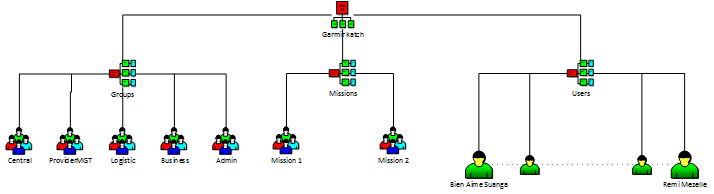
\includegraphics[scale=0.4]{Images/SchemaLDAP.png}
	  \caption{Structure de l'annuaire}
	  \label{SchemaLDAP}
  \end{figure}
 
  \begin{figure}[htbp]
	\centering
	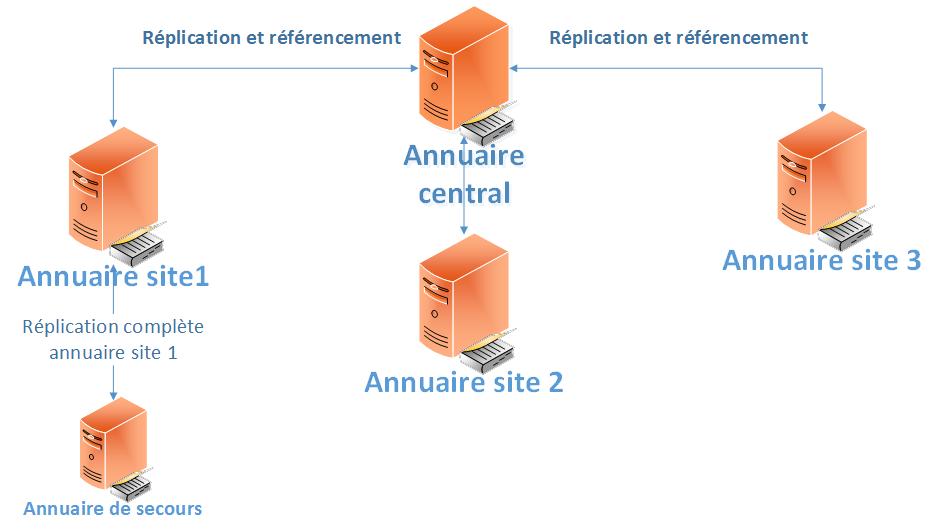
\includegraphics[scale=0.4]{Images/SchemaGlobal.png}
	\caption{Architecture globale}
	\label{SchemaGlobal}
\end{figure}

\begin{figure}[htbp]
	\centering
	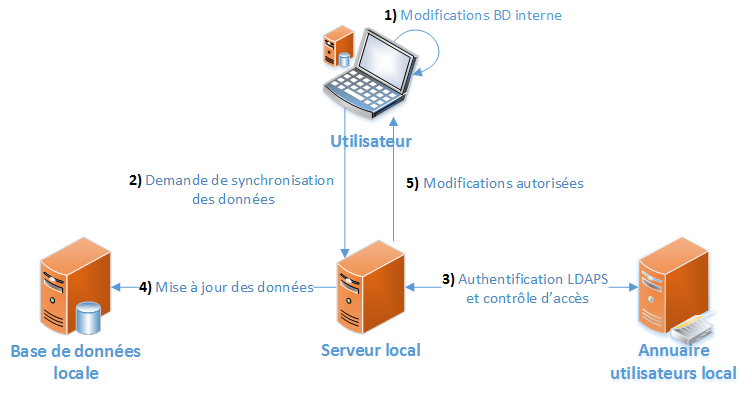
\includegraphics[scale=0.55]{Images/SchemaAuthentification.png}
	\caption{Authentification pour la synchronisation}
	\label{SchemaAuthentification}
\end{figure}

\begin{frame}
  \frametitle{Authentification et contrôle d'accès}
  \begin{block}{\textbf{Droits utilisateurs}}
  \begin{itemize}
  \item Droits pour chaque utilisateur
  \item Droits pour chaque groupe
  \item Autorisations et/ou refus
  \end{itemize}
  \end{block}
\end{frame}

\begin{frame}
  \frametitle{Authentification et contrôle d'accès}
  \begin{block}{\textbf{Gestion des droits}}
  \begin{itemize}
  \item Priorité aux droits directement liés à l'utilisateur 
  \item Priorité aux droits autorisés si l'utilisateur est lié à plusieurs groupes
  \item les droits du groupe
  \end{itemize}
  \end{block}
\end{frame}

\begin{frame}
  \frametitle{Authentification et contrôle d'accès}
  \begin{block}{\textbf{Autres Protocoles connus}}
  \begin{itemize}
  \item RADIUS (Remote Authentication Dial-In User Service)
  \item PAP (Password Authentication Protocol)
  \item MS-CHAP (Microsoft Challenge Handshake Authentication Protocol)
  \item ... 
  \end{itemize}
  \end{block}
%   Utiles si on sait comment se defendre face à une question
%   \begin{block}{\textbf{Quelques normes utiles}}
%   \begin{itemize}
%   \item X500 
%   \item UDDI : Universal Description Discovery and Integration
%   \item TULLEB : Titre Uniforme Labellisé Librement et Édité(Norme destinée aux annuaires publicitaires)
%   \item ... 
%   \end{itemize}
%   \end{block}
\end{frame}

\begin{frame}
  \frametitle{Authentification et contrôle d'accès}
  \begin{block}{\textbf{Travail effectué}}
  \begin{itemize}
  \item Mis en place du serveur 
    \begin{itemize}
    \item Windows
    \item Linux
    \end{itemize}
  \item Ajout d'un schema 
  \item Librairie de consulation via l'outil % à rénomer 
  \end{itemize}
  \end{block}
\end{frame}

\begin{frame}
  \frametitle{Authentification et contrôle d'accès}
  \begin{block}{\textbf{ce qu'il reste à faire}}
  \begin{itemize}
  \item Système de réplication et de référencement 
  \item Ajout et modification dans l'outil
  \end{itemize}
  \end{block}
\end{frame}

\begin{frame}
  \frametitle{Authentification et contrôle d'accès}
  \begin{block}{\textbf{Probleme rencontré }}
  \begin{itemize}
  \item Peu de connaissance de l'architecture LDAP
  \item Recherche des librairies LDAP pour windows 
  \item 
  \end{itemize}
  \end{block}
\end{frame}


\subsection[Tests sur l'interface graphique et unitaires (CdR)]{Tests sur l'interface graphique et unitaires (CdR)}
\begin{frame}
\frametitle{Les tests}
\begin{block}{\textbf{Pourquoi les tests sont importants dans ce projet}}
\begin{itemize}
\item l'outil doit être fiable
\item les fonctionnalités du cahier des charges doivent être opérationnelles
\end{itemize}
\end{block}
\end{frame}

\begin{frame}
\frametitle{}
\begin{block}{\textbf{Différents types de tests ont été réalisé : }}
\begin{itemize}
\item les tests sur l'interface graphique,
\item les tests unitaires,
\item les tests sur le système de gestion de données.
\end{itemize}
\end{block}
\begin{block}{\textbf{Configuration des tests : }}
\begin{itemize}
\item le framework Qt intègre une librairie de test : QTestlib
\item les tests sont lancés à partir de l'éxecutable
\item différentes options permettent de lancer les différents tests ( \emph{-testldap} )
\end{itemize}
\end{block}
\end{frame}

\begin{block}{\textbf{Test d'un champ sur l'onglet Réquisition }}
\begin{center}
\newcolumntype{R}[1]{>{\raggedleft\arraybackslash }b{#1}}
\newcolumntype{L}[1]{>{\raggedright\arraybackslash }b{#1}}
\newcolumntype{C}[1]{>{\centering\arraybackslash }b{#1}}
\begin{tabular}{|L{2.7cm}|L{7cm}|}
\hline \emph{Cas de test :} & Test-Graphique-08  \\
\hline \emph{Titre :} & testCountryCode   \\
\hline \emph{Objectif :} & Vérifier le bon fonctionnement du champ du code pays dans l'onglet réquisition   \\
\hline \emph{Procédure :} & Cliquer dans le champ du code pays, le remplir avec une chaîne et vérifier que la chaîne correspond   \\
\hline \emph{Données de test :} & On rempli avec la chaîne ``Fr''   \\
\hline \emph{Config :} & Using QtTest library 5.2.1, Qt 5.2.1   \\
\hline \emph{Résultat :} & PASS   \\
\hline 
\end{tabular} 
\end{center}
\end{block} 

\begin{frame}
\begin{block}{\textbf{Les tests graphiques permettent de }}
\begin{itemize}
\item tester les zones de saisies
\item tester les validateurs
\end{itemize}
\end{block}
\end{frame}

\begin{block}{\textbf{Test d'un champ sur l'onglet Providers }}
\begin{center}
\newcolumntype{R}[1]{>{\raggedleft\arraybackslash }b{#1}}
\newcolumntype{L}[1]{>{\raggedright\arraybackslash }b{#1}}
\newcolumntype{C}[1]{>{\centering\arraybackslash }b{#1}}
\begin{tabular}{|L{2.7cm}|L{7cm}|}
\hline \emph{Cas de test :} & Test-Graphique-31  \\
\hline \emph{Titre :} & testWaybillCountryCode   \\
\hline \emph{Objectif :} & Vérifier le bon fonctionnement du champ du code pays du prestataire.   \\
\hline \emph{Procédure :} & Cliquer dans le champ, le remplir avec une chaîne et vérifier que la chaîne correspond   \\
\hline \emph{Données de test :} & On rempli avec la chaîne ``FRA''   \\
\hline \emph{Config :} & Using QtTest library 5.2.1, Qt 5.2.1   \\
\hline \emph{Résultat :} & PASS   \\
\hline 
\end{tabular} 
\end{center}
\end{block}

\begin{frame}
\begin{block}{\textbf{Les tests unitaires de l'annuaire LDAP permettent de}}
\begin{itemize}
\item tester les connexions au serveur
\item tester l'authentification
\item vérifier l'implémentation des groupes
\item tester les droits en\begin{itemize} \item lecture
					  \item écriture
					  \item ajout
					  \item suppression
			  \end{itemize}		
\end{itemize}
\end{block}
\end{frame}

\begin{block}{\textbf{Test d'une connexion à l'annuaire }}
\begin{center}
\newcolumntype{R}[1]{>{\raggedleft\arraybackslash }b{#1}}
\newcolumntype{L}[1]{>{\raggedright\arraybackslash }b{#1}}
\newcolumntype{C}[1]{>{\centering\arraybackslash }b{#1}}
\begin{tabular}{|L{2.7cm}|L{7cm}|}
\hline \emph{Cas de test :} & Test-Unitaire-01  \\
\hline \emph{Titre :} & testConnection   \\
\hline \emph{Objectif :} & Vérifier une connexion à l'annuaire LDAP   \\
\hline \emph{Procédure :} & Initialisation d'une connexion avec un nom d'hôte et un port existant   \\
\hline \emph{Données de test :} & hostname : localhost, port : 389   \\
\hline \emph{Résultat :} & PASS   \\
\hline 
\hline \emph{Cas de test :} & Test-Unitaire-02  \\
\hline \emph{Titre :} & testConnectionBadHostname   \\
\hline \emph{Objectif :} & Vérifier une connexion à l'annuaire LDAP   \\
\hline \emph{Procédure :} & Initialisation d'une connexion avec un faux nom d'hôte et un port existant   \\
\hline \emph{Données de test :} & hostname : toto, port : 389   \\
\hline \emph{Résultat :} & FAIL comme prévu   \\
\hline 
\end{tabular} 
\end{center}
\end{block}

\begin{frame}
\begin{block}{\textbf{Tous les tests sont visualisables dans le cahier des recettes}}
\end{block}
\end{frame}




\subsection[Procédure de déploiement et d'installation (PIT)]{Procédure de déploiement et d'installation (PIT)}
\begin{frame}
\end{frame}

\section[Conclusion]{Conclusion}

\subsection[Conclusion]{Conclusion}
\begin{frame}
	\transdissolve[duration=0.2]<1->
	\frametitle{Conclusion}
\end{frame}

\subsection[Questions~?]{Questions~?}
\begin{frame}
	\transdissolve[duration=0.2]<1->
	\frametitle{Merci de votre attention}
\end{frame}

\end{document}